\documentclass[tikz]{article}
\usepackage[left=1.8cm,right=3cm,top=1.5cm,bottom=2cm]{geometry} % page
% settings
\usepackage{multicol} 
\usepackage{amsmath} % provides many mathematical environments & tools

\DeclareMathOperator{\Var}{Var}
\DeclareMathOperator{\Cov}{Cov}
\DeclareMathOperator{\E}{E}

\usepackage{dsfont}
\usepackage{upgreek}

\usepackage{scalerel}
\def\stretchint#1{\vcenter{\hbox{\stretchto[440]{\displaystyle\int}{#1}}}}

\usepackage[english]{babel}
\usepackage[doument]{ragged2e}

\usepackage{tikz}
\tikzset{
  every point/.style = {radius={\pgflinewidth}, opacity=1, draw, solid, fill=white},
  pt/.pic = {
    \begin{pgfonlayer}{foreground}
      \path[every point, #1] circle;
    \end{pgfonlayer}
  },
  point/.style={insert path={pic{pt={#1}}}}, point/.default={},
  colored point/.style = {point={fill=#1}},
  point name/.style = {insert path={coordinate (#1)}}
}

% Images
\usepackage{graphicx}
\usepackage{float}
\usepackage{subfigure} % subfiguras
\usepackage{caption}
\captionsetup[table]{labelformat=empty}
\captionsetup[figure]{labelformat=empty}

\usepackage{listings}
\usepackage{xcolor}
\definecolor{gray}{rgb}{0.5,0.5,0.5}
\definecolor{darkturquoise}{rgb}{0,0.5,0.5}
\newcommand{\n}[1]{{\color{gray}#1}}
\lstset{numbers=left,numberstyle=\small\color{gray}}

\selectlanguage{english}
\usepackage[utf8]{inputenc}
\setlength{\parindent}{0mm}

\begin{document}

\title{Ejercicios propuestos: Parte III}
\author{David Cabezas Berrido}
\date{}
\maketitle

\section*{Ejercicio 1}

Función masa de probabilidad:

\begin{center}
\begin{tabular}{|c|c c|}
\hline
\multicolumn{1}{|c|}{$X / Y$}& 0& 2\\\hline
  2      & 1/16 & 1/16 \\
  4      & 1/8 & 1/4 \\
  6 & 0 & 1/2 \\ \hline
    
\end{tabular}
\end{center}

\vspace{3mm}

Se pide calcular la función generatriz de momentos y, a partir de
ella, la matriz de covarianzas.

\vspace{5mm}

\textbf{f.g.m.:}
\[M(t_1,t_2) = E[e^{t_1x+t_2y}] = \frac{1}{16}e^{2t_1} +
  \frac{1}{16}e^{2t_1+2t_2} + \frac{1}{8}e^{4t_1} +
  \frac{1}{4}e^{4t_1+2t_2} + \frac{1}{2}e^{6t_1+2t_2} =
  \frac{1}{16}(e^{2t_1} + e^{2t_1+2t_2} + 2e^{4t_1} + 4e^{4t_1+2t_2}
  + 8e^{6t_1+2t_2})\]

\vspace{2mm}

Queremos calcular la \textbf{matriz de covarianzas}

\begin{center}
  $
  \begin{pmatrix}
    \Var(X) & \Cov(X,Y) \\
    \Cov(X,Y) & \Var(Y) 
  \end{pmatrix}
  =
  \begin{pmatrix}
    \mu_{20} & \mu_{11} \\
    \mu_{11} & \mu_{02} 
  \end{pmatrix}
  $
\end{center}

\vspace{2mm}

Para hallar los momentos centrados, podemos hallar primero los no
centrados. Usaremos la función generatriz de momentos para hallarlos.

\[m_{10} = \frac{\partial M}{\partial t_1}(t_1,t_2)\Big|_{t_1=t_2=0} =
  \frac{1}{16}(2e^{2t_1} + 2e^{2t_1+2t_2} + 8e^{4t_1} +
  16e^{4t_1+2t_2} + 48e^{6t_1+2t_2})\Big|_{t_1=t_2=0} =
  \frac{2+2+8+16+48}{16} = \frac{19}{4}\]

\[m_{01} = \frac{\partial M}{\partial t_2}(t_1,t_2)\Big|_{t_1=t_2=0} =
  \frac{1}{16}(2e^{2t_1+2t_2} + 8e^{4t_1+2t_2} +
  16e^{6t_1+2t_2})\Big|_{t_1=t_2=0} = \frac{2+8+16}{16} = \frac{13}{8}\]

\[m_{20} = \frac{\partial^2 M}{\partial
    t_1^2}(t_1,t_2)\Big|_{t_1=t_2=0} = \frac{1}{16}(4e^{2t_1} +
  4e^{2t_1+2t_2} + 32e^{4t_1} + 64e^{4t_1+2t_2} +
  288e^{6t_1+2t_2})\Big|_{t_1=t_2=0} = \frac{4+4+32+64+288}{16} =
  \frac{49}{2}\]

\[m_{02} = \frac{\partial^2 M}{\partial
    t_2^2}(t_1,t_2)\Big|_{t_1=t_2=0} = \frac{1}{16}(4e^{2t_1+2t_2} +
  16e^{4t_1+2t_2} + 32e^{6t_1+2t_2})\Big|_{t_1=t_2=0} =
  \frac{4+16+32}{16} = \frac{13}{4}\]

\[m_{11} = \frac{\partial^2 M}{\partial
    t_1t_2}(t_1,t_2)\Big|_{t_1=t_2=0} = \frac{1}{16}(4e^{2t_1+2t_2} +
  32e^{4t_1+2t_2} + 96e^{6t_1+2t_2})\Big|_{t_1=t_2=0} =
  \frac{4+32+96}{16} = \frac{33}{4}\]

\vspace{3mm}

Ya podemos hallar los momentos centrados:
\begin{align*}
  \mu_{20}&=m_{20}-m_{10}^2 = \frac{49}{2} - \Big(\frac{19}{4}\Big)^2 = \frac{31}{16} \\
  \mu_{11}&=m_{11}-m_{10}m_{01} = \frac{33}{4} - \frac{19}{4}\frac{13}{8} = \frac{17}{32} \\
  \mu_{02}&=m_{02}-m_{01}^2 = \frac{13}{4} - \Big(\frac{13}{8}\Big)^2 = \frac{39}{64}
\end{align*}

Por tanto la matriz de covarianzas es

\begin{center}
  $
  \begin{pmatrix}
    \frac{31}{16} & \frac{17}{32} \vspace{2mm}\\
    \frac{17}{32} & \frac{39}{64} 
  \end{pmatrix}
  $
\end{center}

\section*{Ejercicio 2}

Función densidad:
\[f(x,y)=\frac{1}{18} \quad -3<x<3,\ -5<y<-2+x\]

Se pide calcular la recta y la curva de regresión de $Y$ sobre $X$,
así como el coeficiente de determinación lineal y la razón de
correlación.

\begin{center}
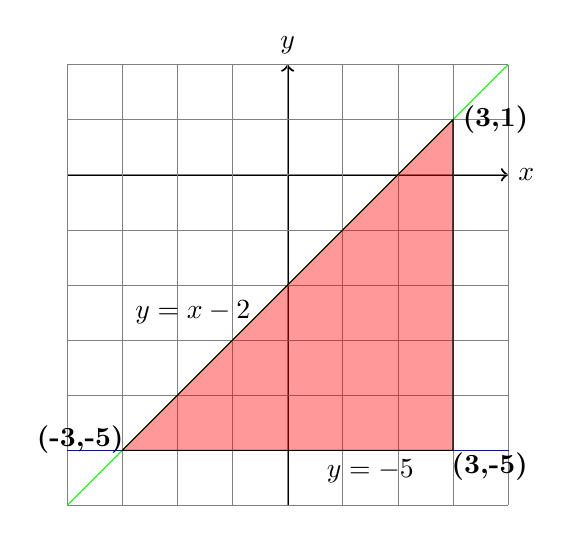
\begin{tikzpicture}[scale=0.7]

  \draw[->,thick] (-4,0) -- (4,0) node[right] {$x$};
  \draw[->,thick] (0,-6) -- (0,2) node[above] {$y$};

  \draw[style=help lines] (-4,-6) grid (4,2);
  
  \draw[domain=-4:4,smooth,variable=\x,blue] plot ({\x},{-5});
  \draw[domain=-4:4,smooth,variable=\x,green] plot ({\x},{\x-2});

   \node at (-2.8,-4.8) [left] {\textbf{(-3,-5)}};
   \node at (2.8,-5.3) [right] {\textbf{(3,-5)}};
   \node at (3,1) [right] {\textbf{(3,1)}};

   \node at (-0.5,-2.5) [left] {$y=x-2$};
   \node at (1.5,-5) [below] {$y=-5$};

  \draw[fill=red, fill opacity=0.4] (-3,-5) -- (3,-5) -- (3,1) -- cycle;
\end{tikzpicture}
\end{center}

\subsection*{Recta de regresión:}

\[Y=aX+b\]

  donde
  
\[a=\gamma_{Y/X}=\dfrac{\Cov(X,Y)}{Var(X)}, \qquad b=\E(Y)-a\E(X)\]

\subsubsection*{Covarianza:}

\[\Cov(X,Y)=\E(XY)-\E(X)\E(Y)\]

\begin{align*}
  \E(XY)&=\int_{-\infty}^{+\infty}\int_{-\infty}^{+\infty}xyf(x,y)dxdy=\int_{-3}^3\int_{-5}^{x-2}\frac{1}{18}xydydx=\frac{1}{18}\int_{-3}^3x\int_{-5}^{x-2}ydydx \\
               &=\frac{1}{18}\int_{-3}^3x\bigg[\frac{y^2}{2}\bigg]_{-5}^{x-2}dx=\frac{1}{18}\int_{-3}^3x\bigg(\frac{(x-2)^2}{2}-\frac{(-5)^2}{2}\bigg)dx=\frac{1}{36}\int_{-3}^3x(x^2-4x+4-25)dx \\
               &=\frac{1}{36}\int_{-3}^3x^3-4x^2-21xdx=\frac{1}{36}\bigg[\frac{x^4}{4}-\frac{4x^3}{3}-\frac{21x^2}{2}\bigg]_{-3}^3=\frac{1}{36}\bigg[\frac{4x^3}{3}\bigg]_3^{-3}=\frac{1}{36}\bigg(\frac{-108}{3}-\frac{108}{3}\bigg) \\
e               &=\frac{-3}{3}-\frac{3}{3}=-2 \\
  ~\\
  \E(X)&=\int_{-\infty}^{+\infty}\int_{-\infty}^{+\infty}xf(x,y)dxdy=\int_{-3}^3\int_{-5}^{x-2}\frac{1}{18}xdydx=\frac{1}{18}\int_{-3}^3x\int_{-5}^{x-2}dydx \\
               &=\frac{1}{18}\int_{-3}^3x(x-2-(-5))dx=\frac{1}{18}\int_{-3}^{3}x^2+3xdx=\frac{1}{18}\bigg[\frac{x^3}{3}+\frac{3x^2}{2}\bigg]_{-3}^3= \\
               &=\frac{1}{18}\bigg(\frac{27}{3}-\frac{-27}{3}\bigg)=1
\end{align*}

\begin{align*}
  \E(Y)&=\int_{-\infty}^{+\infty}\int_{-\infty}^{+\infty}yf(x,y)dxdy=\int_{-3}^3\int_{-5}^{x-2}\frac{1}{18}ydydx=\frac{1}{18}\int_{-3}^3\int_{-5}^{x-2}ydydx \\
              &=\frac{1}{18}\int_{-3}^3\bigg[\frac{y^2}{2}\bigg]_{-5}^{x-2}dx=\frac{1}{36}\int_{-3}^{3}(x-2)^2-(-5)^2dx=\frac{1}{36}\int_{-3}^{3}x^2-4x-21dx \\ &=\frac{1}{36}\bigg[\frac{x^3}{3}-2x^2-21x\bigg]_{-3}^3=\frac{1}{36}\bigg(\frac{27}{3}-63-\Big(\frac{-27}{3}+63\Big)\bigg)=-3
\end{align*}

\[\Cov(X,Y)=\E(XY)-\E(X)\E(Y)=-2-1\dot(-3)=1\]

\subsubsection*{Varianza de X:}

\[\Var(X)=\E(X^2)-\E(X)^2\]

\begin{align*}
  \E(X^2)&=\int_{-\infty}^{+\infty}\int_{-\infty}^{+\infty}x^2f(x,y)dxdy=\int_{-3}^3\int_{-5}^{x-2}\frac{1}{18}x^2dydx=\frac{1}{18}\int_{-3}^3x^2\int_{-5}^{x-2}dydx \\
                &=\frac{1}{18}\int_{-3}^3x^2(x-2-(-5))dx=\frac{1}{18}\int_{-3}^{3}x^3+3x^2dx=\frac{1}{18}\bigg[\frac{x^4}{4}+x^3\bigg]_{-3}^3= \\
                &=\frac{1}{18}\Big(27-(-27)\Big)=3
\end{align*}

\[\Var(X)=\E(X^2)-\E(X)^2=3-1^2=2\]

\subsubsection*{Recta de regresión:}
\[a=\gamma_{Y/X}=\frac{\Cov(X,Y)}{\Var(X)}=\frac{1}{2}\]
\[b=\E(Y)-a\E(X)=-3-1\frac{1}{2}=-\frac{7}{2}\]
\[Y=\frac{1}{2}X-\frac{7}{2}\]

\begin{center}
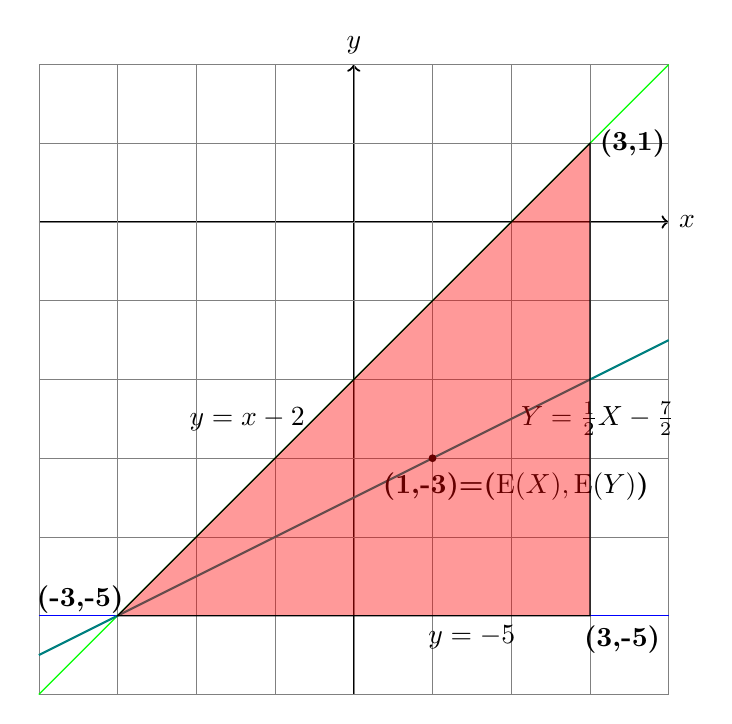
\begin{tikzpicture}[scale=1]

  \draw[->,thick] (-4,0) -- (4,0) node[right] {$x$};
  \draw[->,thick] (0,-6) -- (0,2) node[above] {$y$};

  \draw[style=help lines] (-4,-6) grid (4,2);
  
  \draw[domain=-4:4,smooth,variable=\x,blue] plot ({\x},{-5});
  \draw[domain=-4:4,smooth,variable=\x,green] plot ({\x},{\x-2});
  \draw[domain=-4:4,thick,variable=\x,darkturquoise] plot({\x},{0.5*\x-3.5});
  \node at (-2.8,-4.8) [left] {\textbf{(-3,-5)}};
  \node at (2.8,-5.3) [right] {\textbf{(3,-5)}};
  \node at (3,1) [right] {\textbf{(3,1)}};
  %\node at (1,-3) [below] {~\hspace{20mm}\textbf{(1,-3)=($\E(X),\E(Y)$)}};

  \node at (-0.5,-2.5) [left] {$y=x-2$};
  \node at (1.5,-5) [below] {$y=-5$};
  \node at (2,-2.5) [right] {$Y=\frac{1}{2}X-\frac{7}{2}$};

  \draw (1,-3) node[circle,fill,inner sep=1pt,label=below:~\hspace{20mm}\textbf{(1,-3)=($\E(X),\E(Y)$)}](E){};
  
  \draw[fill=red, fill opacity=0.4] (-3,-5) -- (3,-5) -- (3,1) -- cycle;
\end{tikzpicture}
\end{center}

\subsection*{Coeficiente de determinación lineal:}

\subsection*{Curva de regresión:}
\[Y=\varphi(X)=E(Y/X)\]

\subsubsection*{Esperanza condicionada:}
\[\E(Y/X=x)=\int_{-\infty}^{+\infty}yf(y/X=x)dy\]

Necesito la condicionada de $Y$ a $X$.

\subsubsection*{Marginal:}
\[f_1(x)=\int_{-\infty}^{+\infty}f(x,y)dy=\int_{-5}^{x-2}\frac{1}{18}dy=\frac{1}{18}(x-2-(-5))=\frac{1}{18}(x+3) \qquad x\in]-3,3[\]

\subsubsection*{Condicionada:}
$x\in]-3,3[$
\[f(y/X=x)=\frac{f(x,y)}{f_1(x)}=\frac{\frac{1}{18}}{\frac{1}{18}(x+3)}=\frac{1}{x+3} \qquad y\in]-5,x-2[\]

\subsubsection*{Curva de regresión:}

\begin{align*}
  \E(Y/X=x)&=\int_{-\infty}^{+\infty}yf(y/X=x)dy=\int_{-5}^{x-2}y\frac{1}{x+3}dy=\frac{1}{x+3}\bigg[\frac{y^2}{2}\bigg]_{-5}^{x-2} \\
                  &=\frac{1}{2x+6}\Big((x-2)^2-(-5)^2\Big)=\frac{x^2-4x-21}{2x+6}=\frac{(x+3)(x-7)}{2(x+3)}=\frac{1}{2}x-\frac{7}{2}
\end{align*}

\[Y=\varphi(X)=E(Y/X)=\frac{1}{2}X-\frac{7}{2}\]

En este caso coincide con la recta de regresión.

\subsection*{Razón de correlación:}

\[\eta_{Y/X}^2=\frac{\Var(\E(Y/X))}{\Var(Y)}=1-\frac{\E(\Var(Y/X))}{\Var(Y)}\]

\subsubsection*{Varianza de la esperanza condicionada:}

\[\Var(\E(Y/X))=\E(\E(Y/X)^2)-\E(\E(Y/X))^2\]
\begin{align*}
  \E(\E(Y/X=x)^2)&=\int_{-\infty}^{+\infty}E(Y/X=x)^2f_1(x)dx=\int_{-3}^{3}\frac{1}{4}(x^2-14x+49)\frac{1}{18}(x+3)dx \\
                 &=\frac{1}{72}\int_{-3}^{3}x^3-11x^2+7x+147dx=\frac{1}{72}\bigg[\frac{x^4}{4}-11\frac{x^3}{3}+7\frac{x^2}{2}+147x\bigg]_{-3}^{3} \\
                 &=\frac{1}{72}\bigg(-11\frac{27}{3}+11\frac{-27}{3}+147 \cdot 6\bigg)=\frac{19}{2} \\
  ~ \\
  \E(\E(Y/X))&=\E(Y)=-3                 
\end{align*}
\[\Var(\E(Y/X))=\E(\E(Y/X)^2)-\E(\E(Y/X))^2=\frac{19}{2}-(-3)^2=\frac{1}{2}\]

\newpage

\subsubsection*{Varianza de Y:}

\[\Var(Y)=\E(Y^2)-\E(Y)^2\]

\begin{align*}
  \E(Y^2)&=\int_{-\infty}^{+\infty}\int_{-\infty}^{+\infty}y^2f(x,y)dxdy=\int_{-3}^3\int_{-5}^{x-2}\frac{1}{18}y^2dydx=\frac{1}{18}\int_{-3}^3\int_{-5}^{x-2}y^2dydx \\
         &=\frac{1}{18}\int_{-3}^3\bigg[\frac{y^3}{3}\bigg]_{-5}^{x-2}dx=\frac{1}{54}\int_{-3}^{3}(x-2)^3-(-5)^3dx=\frac{1}{54}\int_{-3}^3x^3-6x^2+12x+117dx \\
         &=\frac{1}{54}\int_{-3}^3-6x^2+117dx=\frac{1}{27}\bigg[-2x^3+117x\bigg]_0^3=\frac{1}{27}(-2\cdot 27+117\cdot 3)=11
\end{align*}

\[\Var(Y)=\E(Y^2)-\E(Y)^2=11-(-3)^2=2\]

\subsubsection*{Razón de correlación:}

\[\eta_{Y/X}^2=\frac{\Var(\E(Y/X))}{\Var(Y)}=\frac{\frac{1}{2}}{2}=\frac{1}{4}\]

\end{document}